\documentclass[11pt, oneside]{article}   	% use "amsart" instead of "article" for AMSLaTeX format
\usepackage{geometry}                		% See geometry.pdf to learn the layout options. There are lots.
\geometry{letterpaper}  
\usepackage{amsmath}
                 		% ... or a4paper or a5paper or ... 
%\geometry{landscape}                		% Activate for rotated page geometry
%\usepackage[parfill]{parskip}    		% Activate to begin paragraphs with an empty line rather than an indent
\usepackage{graphicx}				% Use pdf, png, jpg, or eps§ with pdflatex; use eps in DVI mode
								% TeX will automatically convert eps --> pdf in pdflatex		
\usepackage{amssymb}
\usepackage{epstopdf}

%SetFonts

%SetFonts


\title{Commutative Algebra at 17 Gauss Way}
\author{David Eisenbud}
%\date{}							% Activate to display a given date or no date
%goal: 1500 words,  pictures
\begin{document}
\maketitle


The current program on Commutative Algebra at SLMath follows three others; a three-week microprogram in 1987 and year-long programs in 2002-03 and 2012-13. Many of the senior participants in the current program were graduate students or postdocs in the earlier ones, and the cumulative effect on the field has been very great.

My first experience at MSRI was during my sabbatical in 1986-87. The 1987 microprogram was a highlight! Led by Mel Hochster, Craig Huneke (who is a current member) and Judith Sally (whose death last month at 86 saddened us all), the program gave the commutative algebraists a taste of how nice it was to be at MSRI. My own experience that year led to my application for the job of Director, 20 years later!

There are perhaps a dozen intertwined themes being pursued in the current semester, from singularities and representation theory in positive characteristic to free resolutions, finite and infinite, a wonderful stew of commutative algebra. Its far too various to describe succinctly, so instead I'll focus on one topic with a long history, \emph{residual intersections}, the study of ``what's left over'' when you subtract one algebraic variety from another. The question arose in at least three quite independent areas over the course of the late 19th and early 20th century, and I'll describe these origins, which all involve  projective varieties over the complex numbers.

\section{The Five Conic Problem: Residual Intersections}

The first appearance of residual intersections remains, to me, the least intuitively reasonable:

In the middle of the 19th century many mathematicians studied the enumerative geometry of plane curves. To get an idea of what this means, consider first an easy problem: How many circles are simultaneously tangent to 3 general circles in the plane? The answer, is illustrated in Figure~\ref{3264Book}: each of the $8 = 2^{3}$ red circles can pass either inside or outside 
of one of the 3 black circles. 

\begin{figure}\label{3264Book}
\centerline {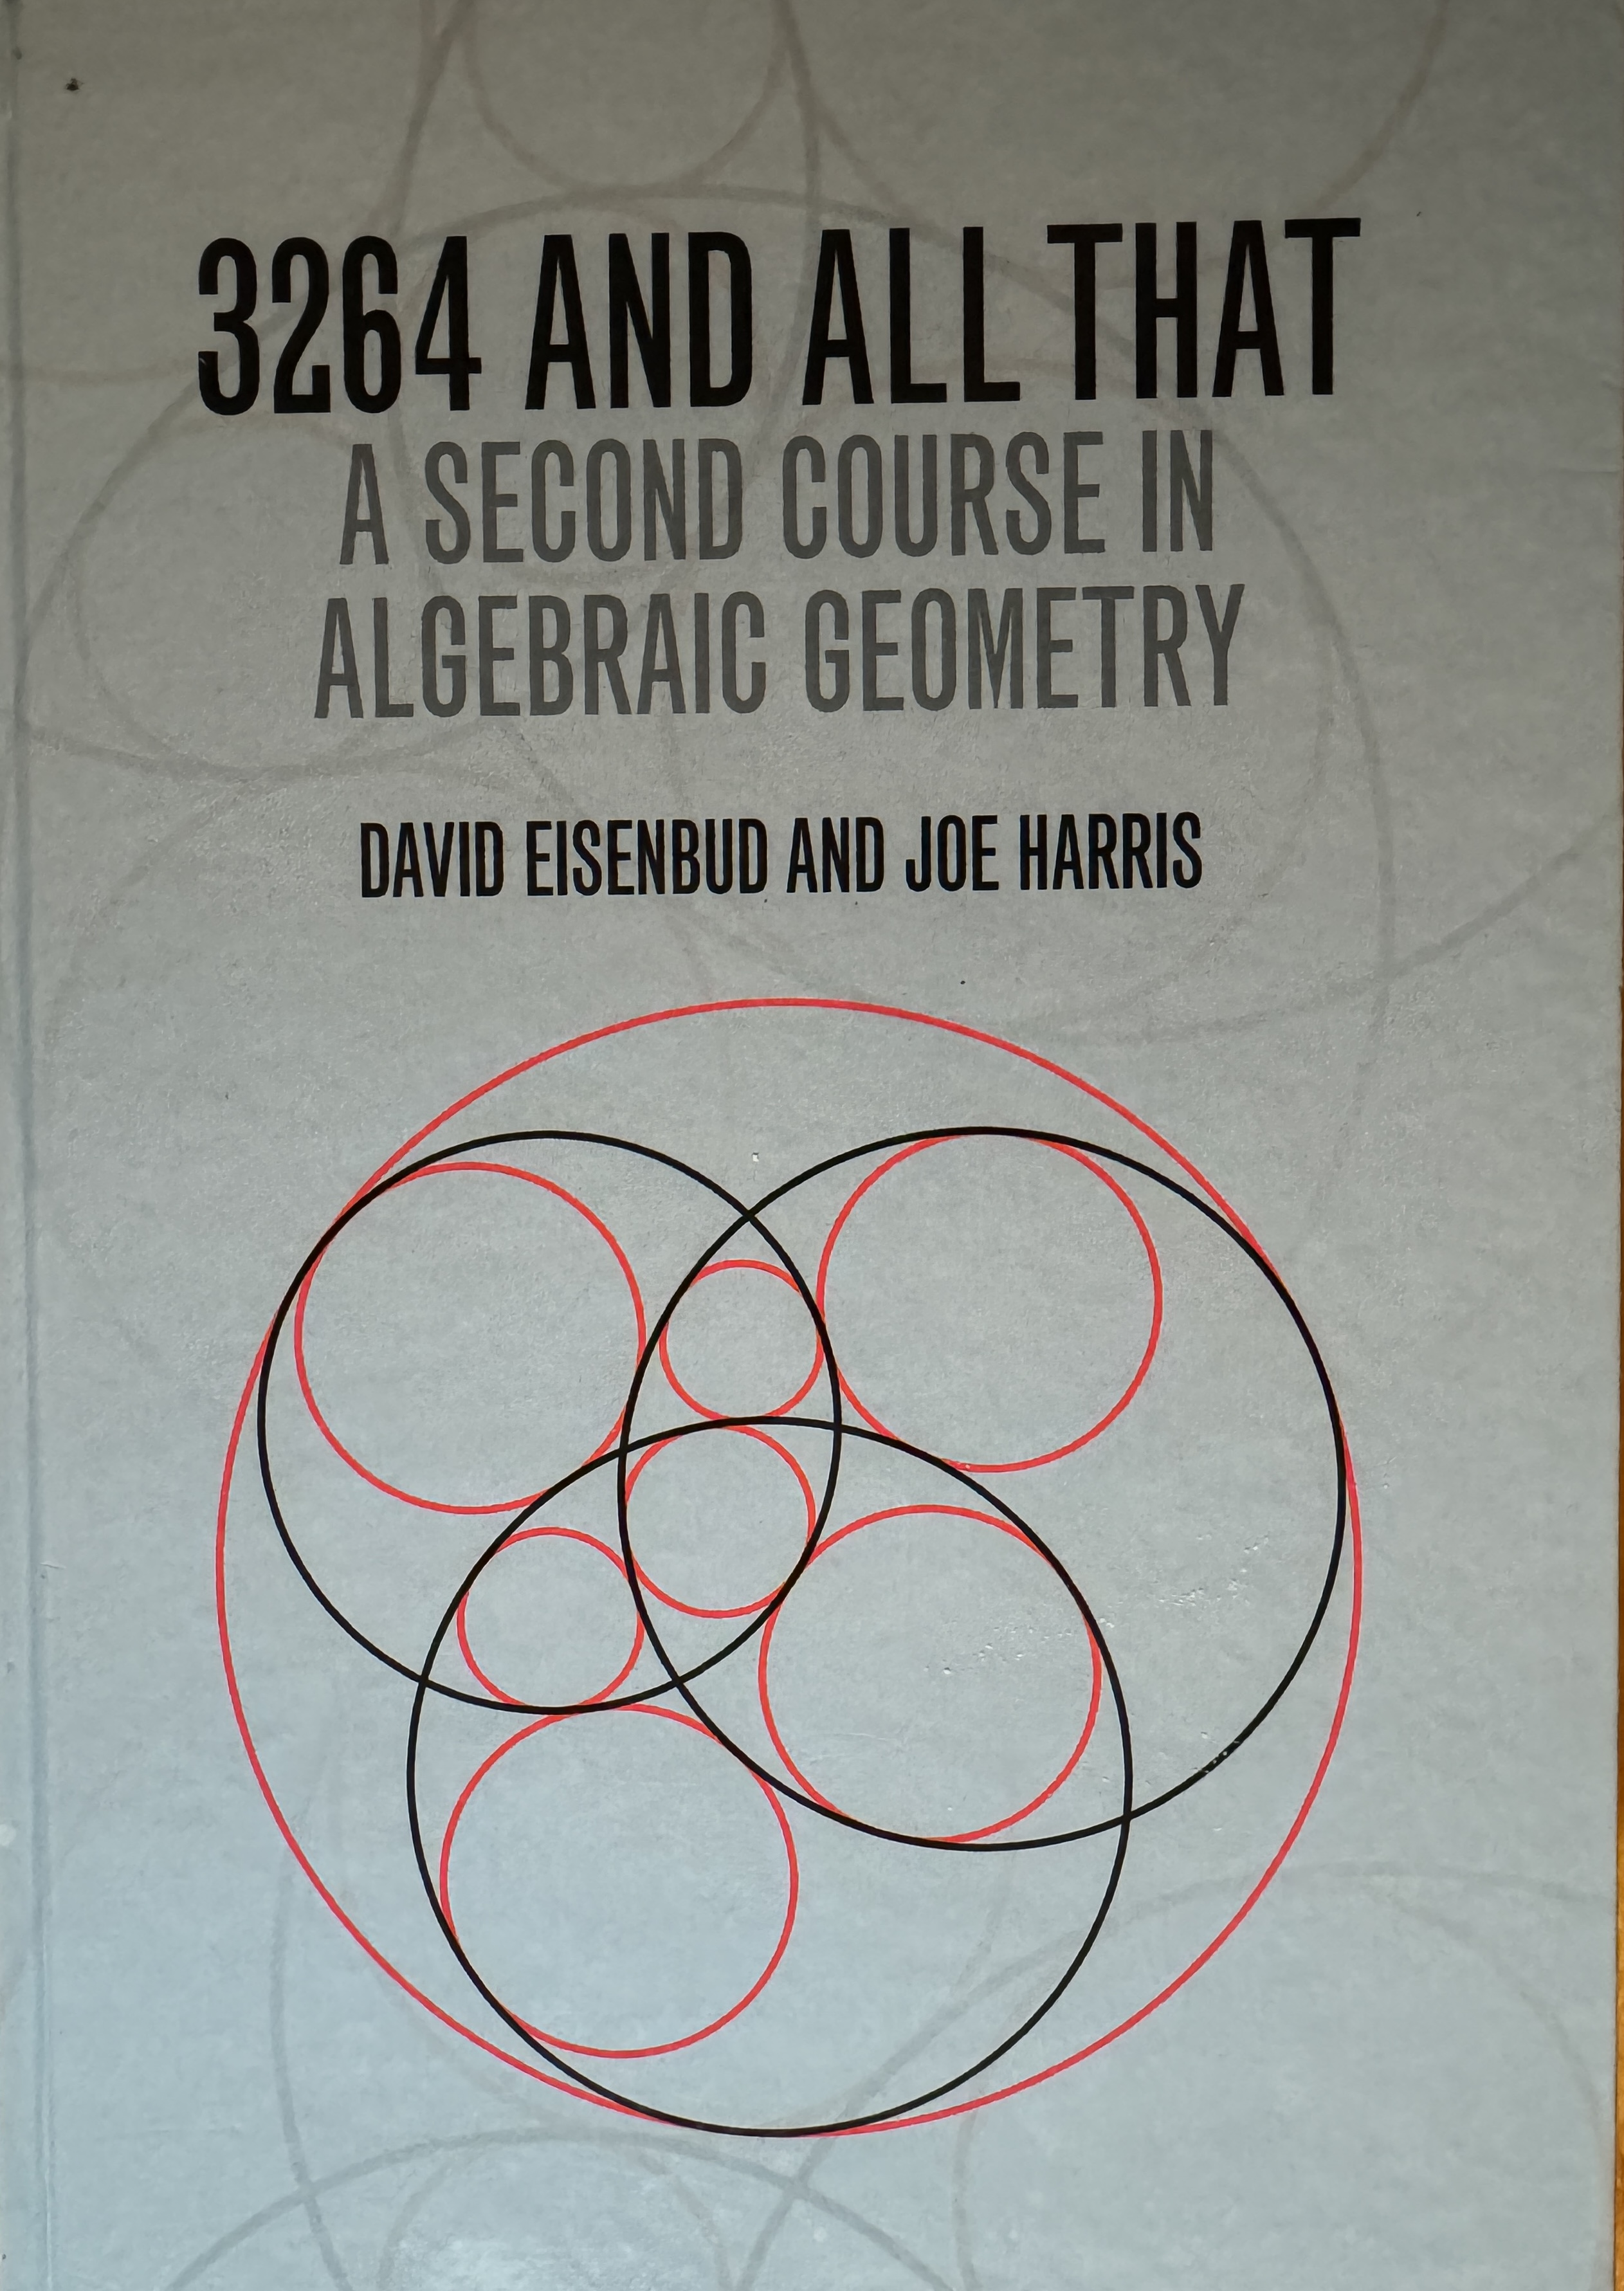
\includegraphics[height=3in]{3264Book.jpg}}
 \caption{There are 8 circles tangent to 3 given circles, as shown on the cover of this recent book
 on intersection theory. The title refers to the Steiner problem, whose solution is given in the book.}
\end{figure}

From a more algebraic point of view, the family of circles is 3-dimensional
(2 dimensions for the center and one for the radius), and the condition on the coefficients of the
equation of a circle $C$ for it to be tangent to a given circle $D$ is a quadratic condition (Proof: fix the center of $C$ and vary just the radius $r$; in general there will be two values of $r$ for which
$C$ is tangent to $D$.) B\'ezout's theorem states that three qadratic surfaces in 3-space generally
meet in 8 points.

In 1848 Jakob Steiner proposed the harder problem: How many plane conics are simultaneously tangent to 5 given general conics? He proposed to answer it by generalizing the argument above: The space of
conics is 5-dimensional (a quadratic equation has 6 coefficients, but a multiple of the equation defines the same conic.) The condition that a conic be tangent to a given conic is an equation of degree 6 on the coefficients, and since there are 5 tangencies required, Steiner reasoned that, by B\'ezout's theorem, the answer should be $6^{5} = 7776$ conics.

This is not correct: the algebraic condition is satisfied by any ``conic''  whose equation is the square of a linear equation, so the equations satisfying the algebraic conditions include an infinite set of ``irrelevant'' solutions. These must be removed to get the correct answer.
How can one count the little parts---points---left over when one has to subtract such a big component, one of the ``wrong'' dimension?
The method, and the correct answer, was discovered by Michel Chasles in 1864 though it would be nearly another 100 years before this was given a rigorous general foundation: there are 3264 ``honest'' conics (in general, smooth) tangent to 5 given general conics. Two different approaches to the proof are explained in the book pictured in 
Figure~\ref{3264Book}.

In fact for a suitable choice of the 5 conics, 
 Ronga, Tognoli, and Vust showed that all the solutions can be represented over the real numbers; 
 some of these are illustrated in Figure~\ref{102Conics}, created by Frank Sottile. 
\begin{figure}\label{102Conics}
\centerline {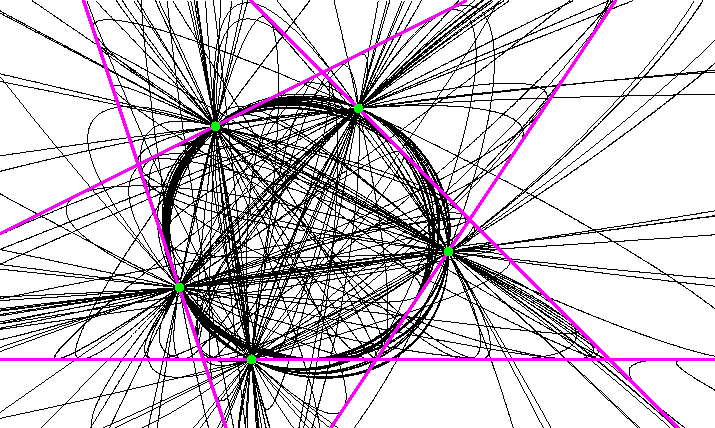
\includegraphics[height=3in]{102_conics.png}}
%\centerline {\includegraphics[height=3in]{102conics.png}}
 \caption{102 of the 3264 conics simultaneously tangent to 5 given conics in 
 a configuration in which all 3264 are defined over the real numbers, due to 
 Frank Sottile. For the construction and the story, see 
 https://franksottile.github.io//research/stories/3264/}
\end{figure}

The natural extension of this idea is to determine the invariants of an algebraic set ``residual'' to another inside a larger algebraic set. Fulton and MacPherson put the geometric theory on a firm foundation in 1978, given certain assumptions about the singularities of the spaces involved. A 1972 paper of Artin and Nagata initiated the study of the singularities of the residual set. Their paper contained a fundamental error, which was soon corrected by Craig Huneke. The field has spawned many problems and theories, and a group at SLMath is currently working on a conjecture that would provide an analogue in all dimensions of part of the results of Gaeta for 3-space.

\section{The Riemann-Roch theorem}
A different manifestation of residual intersections is necessary for the algebraic treatment of the Riemann-Roch theorem. The results of Riemann's famous dissertation in 1851, on what we now call Riemann surfaces, were initially considered
dubious because of his unjustified use of the ``Dirichlet principle'' (and perhaps also because it was simply so far ahead of contemporary thought). First Clebsch and then Brill, (Max) Noether and others undertook to put it on the firm foundation of the algebraic theory of plane curves. One of the terms in the Riemann-Roch theorem involves a difference of divisors, a classic use of residuation. It was Macaulay
who discovered why this works (and a limit of the method), a theory that later blossomed into his theory of "inverse systems".

\section{Curves in 3-space: Linkage} The easiest of the three source problems to understand is historically the latest: How can one classify curves in 3-space? A smooth curve in our sense is the same thing as a Riemann surface, and there are just two topological invariants that characterize such a curve in projective space: its genus $g$ (the number of handles in the Riemann surface) and its degree $d$ (the number of points in which it meets a general plane). So the question becomes: what are the possible pairs $(g,d)$ for a smooth curve in (complex projective) 3-space?

A  smooth curve in 2-space is defined by a single equation and if the degree of the equation is $d$ then the curve is a Riemann surface of genus $d-1\choose 2$.
But already for curves of degree 4 in 3-space, there are two possible genera (0 and 1), so the tight connection between degree and genus is lost.

Suppose first that the ideal of homogeneous polynomials vanishing on $C$ is generated by just 2 of them---the smallest possible number, and that their degrees are $e$ and $f$. In this case,
like that of the plane curves, the genus and degree are determined by $e,f$. For example,
if $e=2$ then $d = 2f$ and $g = (f-1)^{2}$ But there are also a curves of any degree $d$ having genus 0, such as those parameterized by $t \mapsto (t, t^{d-1}, t^{d})$. 

The landscape of curves in 3-space was explored by 
Max Noether (Emmy's father, whom van de Waerden called the ``father of algebraic geometry'') and Georges-Henri Halphen. They jointly received in the Steiner prize of the Prussian Academy of Sciences in 1880 for their work. A primary technique is what is now called \emph{linkage} of curves (also known by its French term liaison):  Given a curve $C$, find two equations from its defining ideal, and look at the ``curve'' $D$ that is defined by these two; in general it will turn out that $D = C\cup C'$, where $C'$ is another smooth curve, said to be \emph{linked} to $C$. A formula from F.S. Macaulay's great paper
of 1913 computes the degree and genus
of $C'$ from that of $C$ and the degrees of the two equations, this gives a way of looking for
new possibilities for $(g,d)$.

The simplest nontrivial case is illustrated by the picture in
Figure~\ref{cubicAndLine}. There the red surface is a cone over a circle, and the yellow surface
is also defined by a quadratic equation. Since both have degree 2, B\'ezout's theorem tells us that the
degree of the intersection ``curve'' will be $2\times 2 = 4$. In the picture it's clear that the vertical line
is part of the intersection; the rest must therefore have degree 3, and in fact it is the \emph{twisted cubic},
parameterizied by $t\mapsto (t, t^{2}, t^{3})$.

\begin{figure}\label{cubicAndLine}
\centerline {\includegraphics[height=5in]{"main/Fig15-1-TwistAndShout"}}
 \caption{A quadratic cone (red) intersecting a smooth quadratic surves (yellow) in the union of a vertical line and a twisted cubic (Picture courtesy of Herwig Hauser, University of Vienna, www.hh.hauser.cc)}
\end{figure}

%In general, if the equations of the two surfaces in the linkage are $s$ and $t$ then it turns out that
%the degrees and genera of $C$ and $C'$ are related by the simple formulas
%\begin{align*}
%&\deg C+\deg C' = st\\
%&g(C) - g({C'}) = \frac{s+t-4}{2}(\deg C-\deg {C'}).
%\end{align*}

The theory of linkage has a long tail! Curves linked (in many steps) to one another are said to be in the same ``linkage equivalence class'', and the curves in 3-space in the linkage class of a line were classified by in the 1940s by Federico Gaeta. A remarkably simple complete algebraic invariant for linkage of curves in 3-space was discovered by Robin Hartshorne and Prabhakar Rao in 1976. 
Meantime, Peskine and Szpiro had rediscovered Macaulay's results, and generalized them to the 
modern setting of Gorenstein local rings. A working group at SLMath is currently trying to
decide whether the closure in projective 3-space of the curve $t \mapsto (t, t^{3}, t^{4})$ is a set-theoretic complete intersection; in other words, is there a self-linked scheme structure on this curve?

There have been many papers refining and generalizing the story since then. An important emphasis of the current SLMath program is centered on a dramatic new understanding of linkage of curves in 4-space and beyond by Jerzy Weyman and his collaborators
Lorenzo Guerrieri and Xianglong Ni, (the latter is a Berkeley graduate student participating in this semester's program).
In contrast to the story for curves in 3-space, now tidily absorbed in the canon of commutative algebra, indicated above, the necessary tools seem to come from the theory of Kac-Moody Lie algebras. It's a shining example of how progress can be made when one field touches a seemingly distant field, as if through a wormhole in the mathematical cosmos! 



\end{document}  

